%\documentclass{beamer}
\documentclass[aspectratio=169]{beamer}
\usetheme{Boadilla}
%\usetheme{Warsaw}
%\setbeamercovered{transparent}
\beamertemplatetransparentcoveredhigh
\usepackage[portuges]{babel}
\usepackage[utf8]{inputenc}
\usepackage[alf]{abntex2cite}	
\usepackage{lmodern}
\usepackage[T1]{fontenc}
\usepackage{hyperref} 
\usepackage{listings}
\usepackage{color}
\usepackage{caption}
\usepackage[portuguese, linesnumbered, vlined, titlenumbered, ruled]{algorithm2e}
\definecolor{dkgreen}{rgb}{0,0.6,0}
\definecolor{gray}{rgb}{0.5,0.5,0.5}
\definecolor{mauve}{rgb}{0.58,0,0.82}

\lstset{frame=tb,
  language=C,
  aboveskip=3mm,
  belowskip=3mm,
  showstringspaces=false,
  columns=flexible,
  basicstyle={\small\ttfamily},
  numbers=none,
  numberstyle=\tiny\color{gray},
  keywordstyle=\color{blue},
  commentstyle=\color{dkgreen},
  stringstyle=\color{mauve},
  breaklines=true,
  breakatwhitespace=true,
  tabsize=3
}
\title[Recursão]{Recursão\\
   Algoritmos e Estrutura de Dados I}
\author[IEng - UFMT]{Instituto de Engenharia -- UFMT}
%\institute[2020/2]{Segundo Semestre de 2020}
\date{}



\begin{document}

%------------------------------------------------
\begin{frame}

\titlepage % Print the title page as the first slide

\begin{figure}[!h]
  \centering
  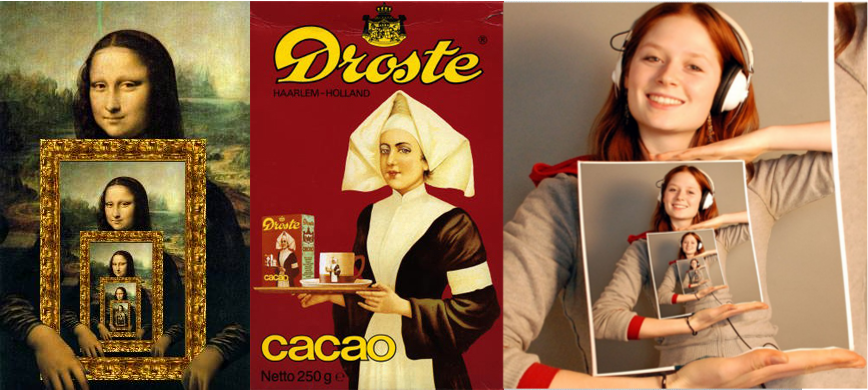
\includegraphics[width=250pt]{imgs/introducao.png}
  \label{fig_introducao}
\end{figure}

\end{frame}

%------------------------------------------------

\begin{frame}
\frametitle{Roteiro} % Table of contents slide, comment this block out to remove it
\tableofcontents % Throughout your presentation, if you choose to use \section{} and \subsection{} commands, these will automatically be printed on this slide as an overview of your presentation
\end{frame}

%----------------------------------------------------------------------------------------
%	PRESENTATION SLIDES
%----------------------------------------------------------------------------------------

%------------------------------------------------
\section{Objetivos}

\begin{frame}
\frametitle{Objetivos}

Esta aula tem como objetivos:

\begin{enumerate}
\item Apresentar processos recursivos;
\item Elucidar os prós e contras da implementação recursiva;
\item Explicitar quando é viável utilizar essa técnica, em termos de desempenho;
\item Exemplificar a implementação de algoritmos recursivos.
\end{enumerate}

\end{frame}


%------------------------------------------------
\section{Introdução} % Sections can be created in order to organize your presentation into discrete blocks, all sections and subsections are automatically printed in the table of contents as an overview of the talk
%------------------------------------------------

\begin{frame}
\frametitle{Introdução}
\begin{block}{Função recursiva}
 Segundo \citeonline{Piva2014}, uma função é dita recursiva quando é definida em termos dela mesma.
\end{block}
\begin{itemize}
\item A recursão está relacionada à indução matemática, sendo formada por um (ou mais) caso base e um passo recursivo;
\item O uso da recursão geralmente permite uma descrição mais clara e concisa dos algoritmos; 
\end{itemize}
\end{frame}

%----------------------------------------------------------------------------------------

\begin{frame}
\frametitle{Introdução}
\begin{itemize}
\item No entanto, mesmo a recursão sendo a forma mais prática de implementar algumas soluções, não é a técnica mais eficiente;
\item É importante saber quando utilizar a recursão e quando não utilizar;
\item Para entender a técnica, vamos começar por um exemplo simples.
\end{itemize}

\end{frame}


%------------------------------------------------
\section{Exemplo 1: Fatorial} 
%------------------------------------------------

\begin{frame}
\frametitle{Exemplo: Fatorial}
 Considere o fatorial de um inteiro positivo $n$, em que $n!$ é dado pela seguinte fórmula:
\begin{equation*}
    fatorial(n) = \begin{cases}
               1                & \text{se } n = 0 \\
               n \times fatorial(n-1) & \text{se } n > 0 
           \end{cases}
\end{equation*}
\begin{itemize}
\pause
\item Essa definição estabelece um processo recursivo para calcular o fatorial de um inteiro $n$.
\item O caso trivial ocorre quando $n = 0$;
\item Assim, usando-se esse processo recursivo, o cálculo de $5!$, por exemplo, é feito como a seguir:
\end{itemize}

\end{frame}

%------------------------------------------------

\begin{frame}
\frametitle{Exemplo: Fatorial}

\begin{figure}[!h]
  \centering
  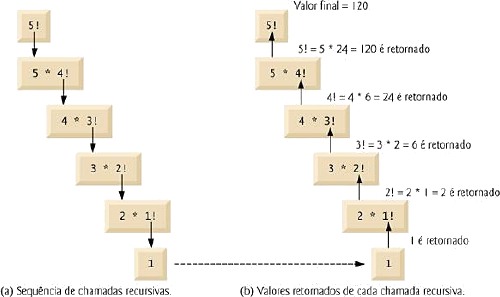
\includegraphics[width=250pt]{imgs/exemplo1_fatorial.png}
  \caption{\footnotesize{Adaptada de \citeonline{Deitel2010}.}}
  \label{fig_exemplo_fatorial}
\end{figure}
\end{frame}

%------------------------------------------------

\begin{frame}[fragile]
\frametitle{Exemplo: Fatorial}
% \scalebox{0.5}{
\begin{algorithm}[H]
\caption{fatorial} 
\label{fatorial}
\Entrada{$n$}
\Saida{$n!$}
\Inicio{
  \Se { ($n = 0$) } {
    \Retorna $1$
    }
  \Senao {
    \Retorna $n \times fatorial (n - 1)$
  } 
}
\end{algorithm}
% }   
\end{frame}

%------------------------------------------------

\begin{frame}[fragile]
\frametitle{Exemplo: Fatorial}
\begin{lstlisting}
int fatorial(int n) {
  if (n == 0)
    return 1;
  else 
    return n*fatorial(n-1);  
}
\end{lstlisting}
\end{frame}

%------------------------------------------------

\begin{frame}[fragile]
\frametitle{Exemplo: Fatorial}
Calcula-se o fatorial de 5 da seguinte forma:

\begin{eqnarray}
 fatorial(5)&=& 5 \times fatorial(5-1) \nonumber \\
	    &=& 5 \times fatorial(4) \nonumber \\
	    &=& 5 \times 4 \times fatorial(4-1) \nonumber \\ 
	    &=& 5 \times 4 \times fatorial(3) \nonumber \\ 
	    &=& 5 \times 4 \times 3 \times fatorial(3-1) \nonumber \\
            &=& 5 \times 4 \times 3 \times fatorial(2) \nonumber \\
	    &=& 5 \times 4 \times 3 \times 2 \times fatorial(2-1) \nonumber \\
	    &=& 5 \times 4 \times 3 \times 2 \times fatorial(1) \nonumber \\
	    &=& 5 \times 4 \times 3 \times 2 \times 1 \times fatorial(1-1) \nonumber \\
	    &=& 5 \times 4 \times 3 \times 2 \times 1 \times fatorial(0) \nonumber \\	    
	    &=& 5 \times 4 \times 3 \times 2 \times 1 \times 1 \nonumber \\
	    &=& 120 \nonumber
\label{calculo_fatorial}	    
\end{eqnarray}
\end{frame}

%----------------------------------------------------------------------------------------
\section{Exemplos}
%----------------------------------------------------------------------------------------

\begin{frame}
\frametitle{Exemplo: Somatória}
Implemente um algoritmo que calcule o valor da soma dos números de 1 a $n$ de forma recursiva.
\end{frame}

%------------------------------------------------

\begin{frame}[fragile]
\frametitle{Exemplo: Somatória}
\begin{lstlisting}
int somatoria(int n) {
  if (n == 0)
    return 0;
  else 
    return n + somatoria(n-1);
}
\end{lstlisting}
\end{frame}

%------------------------------------------------

\begin{frame}[fragile]
\frametitle{Exemplo: Somatória}
Calcula-se a soma de 1 até 3, ou seja $somatoria(3)$, da seguinte forma

\begin{eqnarray}
 somatorio(3)&=& 3 + somatorio(3-1) \nonumber \\
            &=& 3 + somatorio(2) \nonumber \\
	    &=& 3 + 2 + somatorio(2-1) \nonumber \\
	    &=& 3 + 2 + 1 + somatorio(1-1) \nonumber \\
	    &=& 3 + 2 + 1 + 0 \nonumber \\
	    &=& 6. \nonumber 
\end{eqnarray}

\end{frame}
%----------------------------------------------------------------------------------------

\begin{frame}
\frametitle{Exemplo: Multiplicação}
Implemente um algoritmo que calcule o valor da multiplicação de dois números, $x$ e $y$, de forma recursiva, utilizando apenas soma.
\end{frame}

%------------------------------------------------

\begin{frame}[fragile]
\frametitle{Exemplo: Multiplicação}
\begin{lstlisting}
int multiplicacao(int x, int y) {
  if (y == 0)
    return 0;
  else
    return x + multiplicacao(x, y-1);
  
}
\end{lstlisting}
\end{frame}

%------------------------------------------------

\begin{frame}[fragile]
\frametitle{Exemplo: Multiplicação}
Calcula-se a multiplicação $4 \times 3$ conforme a equação a seguir.

\begin{eqnarray}
 multiplicacao(4,3)&=& 4 + multiplicacao(4,3-1) \nonumber \\
                &=& 4 + multiplicacao(4,2) \nonumber \\
	        &=& 4 + 4 + multiplicacao(4,2-1) \nonumber \\
	        &=& 4 + 4 + multiplicacao(4,1) \nonumber \\
	        &=& 4 + 4 + 4 + multiplicacao(4,1-1) \nonumber \\
	        &=& 4 + 4 + 4 + multiplicacao(4,0) \nonumber \\ 
	        &=& 4 + 4 + 4 + 0 \nonumber \\
	        &=& 12 \nonumber
\end{eqnarray}
\end{frame}

%----------------------------------------------------------------------------------------

\begin{frame}
\frametitle{Exemplo: Potência}
Implemente um algoritmo que calcule o valor da potência de $x$ elevado a $y$, de forma recursiva.
\end{frame}

%------------------------------------------------

\begin{frame}[fragile]
\frametitle{Exemplo: Potência}
\begin{lstlisting}
int potencia(int x, int y) {
  if (y == 0)
    return 1;  
  if (y == 1)
    return x;
  else 
    return x*potencia(x,y-1);
}
\end{lstlisting}
\end{frame}

%------------------------------------------------

\begin{frame}[fragile]
\frametitle{Exemplo: Potência}
Calcula-se a potência de $4$ elevado a $3$ conforme a equação a seguir.

\begin{eqnarray}
 potencia(4,3)&=& 4 \times potencia(4,3-1) \nonumber \\
                &=& 4 \times potencia(4,2) \nonumber \\
	        &=& 4 \times 4 \times potencia(4,2-1) \nonumber \\
	        &=& 4 \times 4 \times potencia(4,1) \nonumber \\
	        &=& 4 \times 4 \times 4 \nonumber \\
	        &=& 64 \nonumber
\end{eqnarray}
\end{frame}

%----------------------------------------------------------------------------------------

\begin{frame}
\frametitle{Exemplo: Conta dígitos}
Implemente um algoritmo recursivo que dado um número, $n$, informe quantos dígitos $n$ possui.
\end{frame}

%------------------------------------------------

\begin{frame}[fragile]
\frametitle{Exemplo: Conta dígitos}
\begin{lstlisting}
int conta_digitos(int n) {
  if (n < 10)
    return 1;  
  else 
    return 1 + conta_digitos(n/10);
}
\end{lstlisting}
\end{frame}

%------------------------------------------------

\begin{frame}[fragile]
\frametitle{Exemplo: Conta dígitos}
O cálculo da quantidade de dígitos do número $9876$ pode ser verificado na equação abaixo.

\begin{eqnarray}
  conta\_digitos(9876)&=& 1 + conta\_digitos(\frac{9876}{10}) \nonumber \\
                &=& 1 + conta\_digitos(987) \nonumber \\
	        &=& 1 + ( 1 + conta\_digitos(\frac{987}{10}) ) \nonumber \\
	        &=& 1 + ( 1 + conta\_digitos(98) ) \nonumber \\
	        &=& 1 + ( 1 + ( 1 + conta\_digitos(\frac{98}{10} ) ) ) \nonumber \\
	        &=& 1 + ( 1 + ( 1 + conta\_digitos(9) ) ) \nonumber \\
	        &=& 1 + ( 1 + ( 1 + 1 ) ) \nonumber \\
	        &=& 4 \nonumber 
\label{calculo_conta_digitos}
\end{eqnarray}
\end{frame}
%----------------------------------------------------------------------------------------

\begin{frame}
\frametitle{Exemplo: Divisão}
Implemente um algoritmo recursivo que dados dois números, $x$ e $y$, calcule a divisão inteira de $x$ por $y$.
\end{frame}

%------------------------------------------------

\begin{frame}[fragile]
\frametitle{Exemplo: Divisão}
\begin{lstlisting}
int divisao(int x, int y) {
  if (x < y)
    return 0;  
  else 
    return 1 + divisao(x-y,y);
}
\end{lstlisting}
\end{frame}

%------------------------------------------------

\begin{frame}[fragile]
\frametitle{Exemplo: Divisão}
Calcula-se a divisão inteira  $\frac{15}{4}$ conforme a equação a seguir.

\begin{eqnarray}
  divisao(15,4)&=& 1 + divisao(15-4,4) \nonumber \\
                &=& 1 + divisao(11,4) \nonumber \\
	        &=& 1 + 1 + divisao(11-4,4) \nonumber \\
	        &=& 1 + 1 + divisao(7,4) \nonumber \\
	        &=& 1 + 1 + divisao(7-4,4) \nonumber \\
	        &=& 1 + 1 + 1 + divisao(3,4) \nonumber \\
	        &=& 1 + 1 + 1 + 0 \nonumber \\
	        &=& 3\nonumber
\end{eqnarray}
\end{frame}

%----------------------------------------------------------------------------------------

\begin{frame}
\frametitle{Exemplo: Resto da divisão (módulo)}
Implemente um algoritmo recursivo que dados dois números, $x$ e $y$, calcule o resto da divisão inteira de $x$ por $y$.
\end{frame}

%------------------------------------------------

\begin{frame}[fragile]
\frametitle{Exemplo: Resto da divisão(módulo)}
\begin{lstlisting}
int resto(int x, int y) {
  if (x < y)
    return x;  
  else 
    return resto(x-y,y);
}
\end{lstlisting}
\end{frame}

%------------------------------------------------

\begin{frame}[fragile]
\frametitle{Exemplo: Resto da divisão}
Calcula-se o resto da divisão $\frac{15}{4}$, conforme a equação abaixo.

\begin{eqnarray}
  resto(15,4)&=& resto(15-4,4) \nonumber \\
                &=& resto(11,4) \nonumber \\
	        &=& resto(11-4,4) \nonumber \\
	        &=& resto(7,4) \nonumber \\
	        &=& resto(7-4,4) \nonumber \\
	        &=& resto(3,4) \nonumber \\
	        &=& 3 \nonumber
\end{eqnarray}
\end{frame}

%----------------------------------------------------------------------------------------

\begin{frame}
\frametitle{Exemplo: Raiz quadrada}
Implemente um algoritmo recursivo que dado um número $n$, calcule a raiz quadrada inteira de $n$.
\end{frame}

%------------------------------------------------

\begin{frame}[fragile]
\frametitle{Exemplo: Raiz quadrada}
\begin{lstlisting}
int raiz_quadrada(int n, int i) {
  if (i*i<=n)
    return raiz_quadrada(n, i+1);  
  else 
    return i-1;
}
\end{lstlisting}
\end{frame}


%------------------------------------------------

\begin{frame}[fragile]
\frametitle{Exemplo: Raiz quadrada}
O cálculo da raiz quadrada inteira pode ser verificado na equação abaixo.

\begin{eqnarray}
  raiz\_quadrada(16,0)&=& raiz\_quadrada(16,1) \nonumber \\
                &=& raiz\_quadrada(16,2) \nonumber \\
	        &=& raiz\_quadrada(16,3) \nonumber \\
	        &=& raiz\_quadrada(16,4) \nonumber \\
	        &=& raiz\_quadrada(16,5) \nonumber \\
	        &=& 4 \nonumber
\label{calculo_raiz_quadrada}
\end{eqnarray}
\end{frame}

%----------------------------------------------------------------------------------------

\begin{frame}
\frametitle{Exemplo: Raiz $n$-ésima}
Implemente um algoritmo recursivo que dados dois números inteiros, denominados $m$ e $n$, calcule a raiz $n$-ésima inteira de $m$. Para isso, utilize a função recursiva para cálculo da potência.
\end{frame}

%------------------------------------------------
\section{Exemplo 2: Fibonacci} 
%------------------------------------------------

\begin{frame}
\frametitle{Exemplo: Fibonacci}
 O número de Fibonacci $F_{n}$ para $n \geq 0$ é definido da seguinte maneira:
\begin{equation*}
    F_{n} = \begin{cases}
	       0                 & \text{se } n = 0 \\
               1                 & \text{se } n = 1 \\
               F_{n-1} + F_{n-2} & \text{se } n > 1
           \end{cases}
\end{equation*}

\begin{itemize}
\pause
\item Os casos bases ocorrem quando $n = 0$ e $n = 1$;
\item Utilizando o processo recursivo, o cálculo de $F_{3}$, por exemplo, é feito como a seguir:
\end{itemize}
\end{frame}

%------------------------------------------------

\begin{frame}[fragile]
\frametitle{Exemplo: Fibonacci}

\begin{figure}[!h]
  \centering
  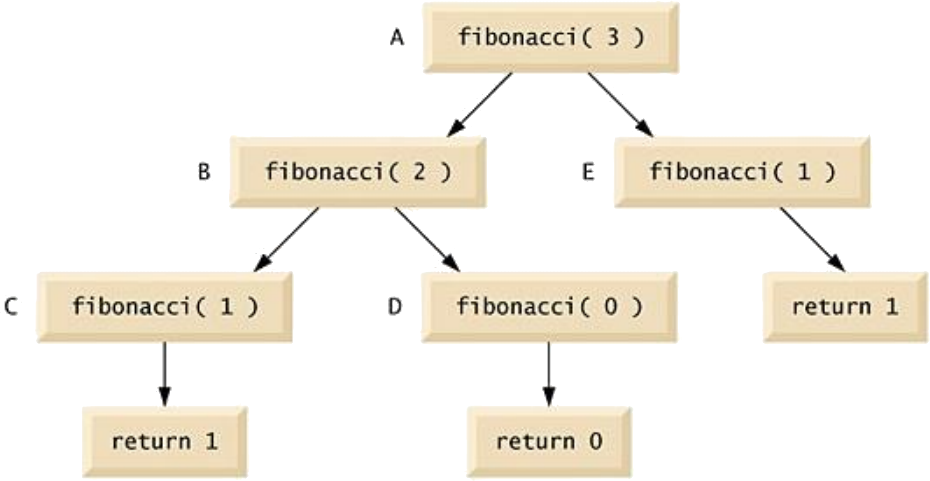
\includegraphics[width=250pt]{imgs/exemplo2_fibonacci.png}
  \caption{\footnotesize{Chamadas de método feitas dentro da chamada fibonacci(3). Adaptada de \citeonline{Deitel2010}.}}
  \label{fig_exemplo_fibonacci1}
\end{figure}
\end{frame}

%------------------------------------------------

\begin{frame}
\frametitle{Exemplo: Fibonacci}

\begin{algorithm}[H]
\caption{fibonacci} 
\label{fibonacci}
\Entrada{$n$}
\Saida{número de Fibonacci $F_{n}$}
\Inicio{
  \Se { ($n = 0$) } {
    \Retorna $0$
    }
  \Se { ($n = 1$) } {
    \Retorna $1$
    }
  \Senao {
    \Retorna $fibonacci(n - 1) + fibonacci (n - 2)$
  } 
}
\end{algorithm}
\end{frame}

%------------------------------------------------

\begin{frame}
\frametitle{Exemplo: Fibonacci}

\begin{figure}[!h]
  \centering
  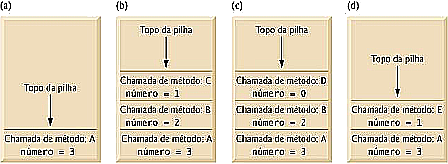
\includegraphics[width=250pt]{imgs/exemplo2_fibonacci_pilha_execucao.png}
  \caption{\footnotesize{Chamadas de método na pilha de execução do programa. Adaptada de \citeonline{Deitel2010}.}}
  \label{fig_exemplo_fibonacci2}
\end{figure}
\end{frame}

%------------------------------------------------

\begin{frame}[fragile]
\frametitle{Exemplo: Fibonacci}
\begin{lstlisting}
int fibonacci(int n) {
  if (n == 0) 
    return 0;
  else if (n == 1)
    return 1;
  else
    return fibonacci(n-1) + fibonacci(n-2);
}
\end{lstlisting}
\end{frame}


%------------------------------------------------
\section{Recursão {\it versus} Iteração} 
%------------------------------------------------
\begin{frame}

Semelhanças

\frametitle{Recursão {\it versus} Iteração}
  \begin{itemize}
    \item Tanto iteração quanto recursão se baseiam em um estrutura de controle: 
      \begin{itemize}
	\item a iteração utiliza estrutura de repetição e recursão utiliza instruções de seleção.
      \end{itemize}
    \item Ambas envolvem repetição:
      \begin{itemize}
	\item a iteração utiliza explicitamente estruturas de repetição e a recursão alcança a repetição por meio de chamadas repetidas de método.
      \end{itemize}    
    \item Ambas envolvem um teste de terminação:
      \begin{itemize}
	\item a iteração quando a condição de repetição falha e a recursão quando o caso base é alcançado.
      \end{itemize}       
    \item Tanto uma quanto a outra podem ocorrer infinitamente.
  \end{itemize}
\end{frame}

%------------------------------------------------

\begin{frame}
\frametitle{Recursão {\it versus} Iteração}
\begin{block}{Soluções iterativas}
 Para ilustrar as diferenças, vamos examinar soluções iterativas para os problemas apresentados.
\end{block}
\end{frame}

%------------------------------------------------

\begin{frame}
\frametitle{Exemplo iterativo: Fatorial}

\begin{algorithm}[H]
\caption{fatorial-iterativo} 
\label{fatorial-iterativo}
\Entrada{$n$}
\Saida{$n!$}
\Inicio{
  $valor \leftarrow 1$\\
  \Para {$i \leftarrow n$ \textrm{at\'{e}} $1$} {
    $valor \leftarrow valor \times i$
  }
  \Retorna $valor$
}
\end{algorithm}

\end{frame}


%------------------------------------------------

\begin{frame}
\frametitle{Exemplo iterativo: Fibonacci}

\begin{algorithm}[H]
\caption{fibonacci-iterativo} 
\label{fibonacci-iterativo}
\Entrada{$n$}
\Saida{número de Fibonacci $F_n$}
\Inicio{
  $f[0] \leftarrow 0$ \\
  $f[1] \leftarrow 1$ \\
  \Para {$i \leftarrow 2$ \textrm{at\'{e}} $n$} {
    $f[i] \leftarrow f[i-1] + f[i-2]$
  }
  \Retorna $f[i]$
}
\end{algorithm}

\end{frame}

%------------------------------------------------
% 
% \begin{frame}
% \frametitle{Quadro comparativo}
% \end{frame}

%------------------------------------------------

\begin{frame}
\frametitle{Recursão {\it versus} Iteração}
A recursão tem muitas negativas:
  \begin{itemize}
    \item Invoca repetidamente o mecanismo, e consequentemente o {\it overhead}, das chamadas de método;
    \item Essa repetição pode ser cara tanto em termos de processador como de espaço de memória;
    \item Cada chamada recursiva faz com que outra cópia do método seja criada;
    \item Esse conjunto de cópias pode consumir espaço considerável de memória;
    \item Como a iteração ocorre dentro de um único método, as chamadas de métodos repetidas e a atribuição extra de memória são evitadas.
  \end{itemize}
\end{frame}


%------------------------------------------------

\begin{frame}
\frametitle{Recursão {\it versus} Iteração}
\begin{block}{Vantagem}
   Então por que escolher recursão?
\end{block}
\pause
\begin{block}{Exemplo}
   Vamos verificar o porquê através de um exemplo.
\end{block}
\end{frame}

%------------------------------------------------
\section{Exemplo 3: Torres de Hanói} 
%------------------------------------------------

\begin{frame}
\frametitle{Exemplo: Torres de Hanói}
  Neste problema, deve-se mover uma pilha de discos de um pino para outro.
  Ao mover a pilha de um pino para outro deve-se ficar atento às restrições:
  \begin{itemize}
   \item um único disco é movido por vez;
   \item em nenhuma circunstância um disco maior pode ser colocado em cima de um disco menor.
  \end{itemize}
  Três pinos são fornecidos e um deles é utilizado para armazenar discos temporariamente.
\begin{figure}[!h]
  \centering
  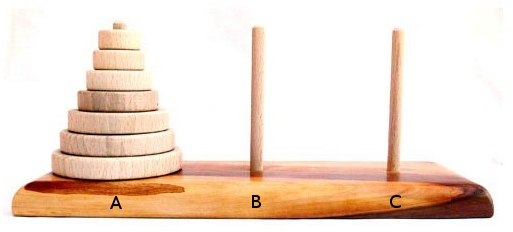
\includegraphics[width=200pt]{imgs/torre_hanoi.png}
  \label{fig_torre_hanoi1}
\end{figure}
\end{frame}

%------------------------------------------------

\begin{frame}
\frametitle{Exemplo: Torres de Hanói}
  \begin{itemize}
  \item Vamos desenvolver um algoritmo que, dada uma entrada que indica a quantidade de discos, informa a sequência de movimentos e quantos são necessários para mover os discos do pino A para o pino C, utilizando o pino B para armazenamento temporário. 
  \item Se o valor fornecido para o programa for $n = 3$, então a sequência de chamadas e as saídas geradas são:  
  \end{itemize}
\end{frame}

%------------------------------------------------

\begin{frame}
\frametitle{Exemplo: Torres de Hanói}

\begin{figure}[!h]
  \centering
  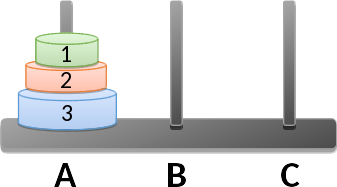
\includegraphics[width=180pt]{imgs/exemplo_torre_hanoi1.png}
  \label{fig_torre_hanoi2}
\end{figure}
\end{frame}

%------------------------------------------------

\begin{frame}
\frametitle{Exemplo: Torres de Hanói}

\begin{figure}[!h]
  \centering
  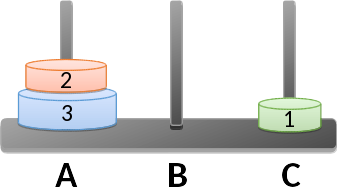
\includegraphics[width=180pt]{imgs/exemplo_torre_hanoi2.png}
  \label{fig_torre_hanoi3}
\end{figure}
Movimento 1: disco 1 do pino A para o pino B.
\end{frame}

%------------------------------------------------

\begin{frame}
\frametitle{Exemplo: Torres de Hanói}

\begin{figure}[!h]
  \centering
  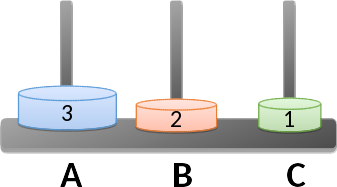
\includegraphics[width=180pt]{imgs/exemplo_torre_hanoi3.png}
  \label{fig_torre_hanoi4}
\end{figure}
Movimento 2: disco 2 do pino A para o pino C.
\end{frame}

%------------------------------------------------

\begin{frame}
\frametitle{Exemplo: Torres de Hanói}

\begin{figure}[!h]
  \centering
  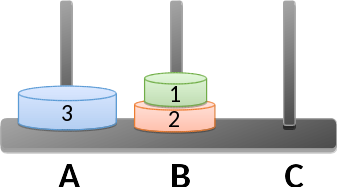
\includegraphics[width=180pt]{imgs/exemplo_torre_hanoi4.png}
  \label{fig_torre_hanoi5}
\end{figure}
Movimento 3: disco 1 do pino C para o pino C.
\end{frame}

%------------------------------------------------

\begin{frame}
\frametitle{Exemplo: Torres de Hanói}

\begin{figure}[!h]
  \centering
  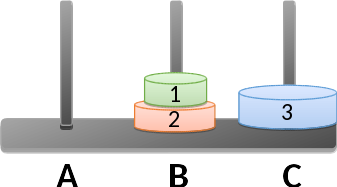
\includegraphics[width=180pt]{imgs/exemplo_torre_hanoi5.png}
  \label{fig_torre_hanoi6}
\end{figure}
Movimento 4: disco 3 do pino A para o pino C.
\end{frame}

%------------------------------------------------

\begin{frame}
\frametitle{Exemplo: Torres de Hanói}

\begin{figure}[!h]
  \centering
  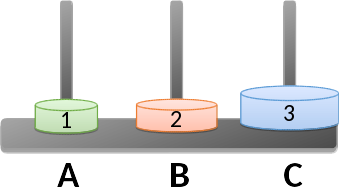
\includegraphics[width=180pt]{imgs/exemplo_torre_hanoi6.png}
  \label{fig_torre_hanoi7}
\end{figure}
Movimento 5: disco 1 do pino B para o pino A.
\end{frame}

%------------------------------------------------

\begin{frame}
\frametitle{Exemplo: Torres de Hanói}

\begin{figure}[!h]
  \centering
  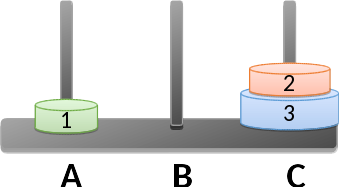
\includegraphics[width=180pt]{imgs/exemplo_torre_hanoi7.png}
  \label{fig_torre_hanoi8}
\end{figure}
Movimento 6: disco 2 do pino B para o pino C.
\end{frame}

%------------------------------------------------

\begin{frame}
\frametitle{Exemplo: Torres de Hanói}

\begin{figure}[!h]
  \centering
  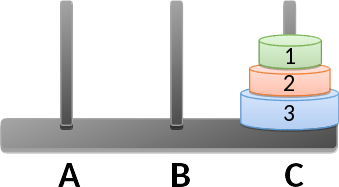
\includegraphics[width=180pt]{imgs/exemplo_torre_hanoi8.png}
  \label{fig_torre_hanoi9}
\end{figure}
Movimento 7: disco 1 do pino A para o pino C.
\end{frame}

%------------------------------------------------

\begin{frame}
\frametitle{Exemplo: Torres de Hanói}
Mover $n$ discos pode ser visualizado em termos de mover $n-1$ discos como a seguir:
\begin{itemize}
 \item Mova $n-1$ discos do pino A para o pino B, utilizando o pino C para armazenamento temporário;
 \item Mova o último disco (o maior) do pino A para o pino C;
 \item Mova os $n-1$ discos do pino B para o pino C, utilizando o pino A para armazenamento temporário.
\end{itemize}
\end{frame}

%------------------------------------------------

\begin{frame}
\frametitle{Exemplo: Torres de Hanói}

\scalebox{0.8}{

\begin{algorithm}[H]
\caption{torres-hanoi($n$, $P_o$, $P_d$, $P_{tmp}$)} 
\label{torres-hanoi}
\Entrada{quantidade $n$ de discos, pino de origem $P_o$, pino de destino $P_d$ e pino auxiliar $P_{tmp}$}
\Saida{sequência e quantidade de movimentos para mover os $n$ discos do pino $P_o$ para o pino $P_d$ utilizando o pino auxiliar $P_{tmp}$. }
\Inicio{
  \CommentSty{// Variável global que indica a ordem de cada movimento na sequência de resolução.}  \\
  global $ordem \leftarrow 0$ \\
  \Se {$n = 1$} {
    Imprimir: \textrm{$ordem$: disco do pino $P_o$ para o pino $P_d$} \\
  }
  torres-hanoi($n-1$, $P_o$, $P_{tmp}$, $P_d$) \\
  Imprimir: \textrm{$ordem$: disco do pino $P_o$ para o pino $P_d$} \\
  torres-hanoi($n-1$, $P_{tmp}$, $P_d$, $P_o$) \\
}
\end{algorithm}
} %\scalebox
\end{frame}

%------------------------------------------------

\begin{frame}
\frametitle{Exemplo: Torres de Hanói}
\begin{itemize}
  \item A quantidade mínima de movimentos $m$ é dada por: $m = 2^n - 1$, em que $n$ é a quantidade de discos;
  \item Ao tentar encontrar uma solução iterativa para esse problema, é provável que nos encontremos irremediavelmente ``amarrados'' no gerenciamento dos discos;
\end{itemize}
\end{frame}


%------------------------------------------------
\section{Exemplo} 
%------------------------------------------------

\begin{frame}
\frametitle{Tarefa}
\begin{block}{Exemplo}
   Escrever um programa em linguagem C que calcula o movimento de $n$ discos de acordo com as regras estabelecidas.
\end{block}
\end{frame}

%------------------------------------------------

\section{Referências bibliográficas}
  \frame{\frametitle{Referências bibliográficas}
    \bibliographystyle{abntex2-alf}
    \bibliography{referencias}
  }

%------------------------------------------------

\begin{frame}
\Huge{\centerline{FIM}}

\begin{figure}[!h]
  \centering
  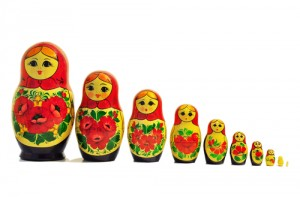
\includegraphics[width=150pt]{imgs/russian_dolls.jpg}
  \label{fig_fim}
\end{figure}

\end{frame}

%----------------------------------------------------------------------------------------

\begin{frame}
  \frametitle{Fim}
\begin{center}
\Huge Fim
\end{center}
\end{frame}

\end{document} 